%% LyX 2.0.2 created this file.  For more info, see http://www.lyx.org/.
%% Do not edit unless you really know what you are doing.
\documentclass[12pt,twoside,english]{report}
\usepackage{lmodern}
\renewcommand{\familydefault}{\rmdefault}
\usepackage[T1]{fontenc}
\usepackage[latin9]{inputenc}
\usepackage[a4paper]{geometry}
\geometry{verbose,tmargin=3.5cm,bmargin=3cm,lmargin=3.5cm,rmargin=3cm,footskip=1cm}
\usepackage{fancyhdr}
\pagestyle{fancy}
\setcounter{secnumdepth}{3}
\setcounter{tocdepth}{3}
\setlength{\parskip}{\medskipamount}
\setlength{\parindent}{0pt}
\usepackage{float}
\usepackage{textcomp}
\usepackage{graphicx}
\usepackage{setspace}
\usepackage[authoryear]{natbib}
\usepackage{nomencl}
% the following is useful when we have the old nomencl.sty package
\providecommand{\printnomenclature}{\printglossary}
\providecommand{\makenomenclature}{\makeglossary}
\makenomenclature
\setstretch{1.5}

\makeatletter
%%%%%%%%%%%%%%%%%%%%%%%%%%%%%% User specified LaTeX commands.
\usepackage{fancyhdr}
\pagestyle{fancy}
\fancyhead[RE]{\bfseries \nouppercase\leftmark}
\fancyhead[LO]{\bfseries \nouppercase \rightmark}

\renewcommand{\chaptermark}[1]{%
\markboth{\chaptername 
\ \thechapter\ }{}}

 
\fancyhead[LE,RO]{\bfseries\thepage}
\fancyfoot{}
\raggedbottom
\setlength{\parindent}{8mm}

\makeatother

\usepackage{babel}
\begin{document}

\chapter{Literature Review\label{chap:Optim-Literature-Review}}

\newpage{}


\section*{Summary}

\noindent This chapter gives an overview of how optimisation techniques
are utilised in the renewable energy literature. A review of the Genetic
Algorithm \nomenclature{GA}{Genetic Algorithm}(GA) technique and
its use in renewable electricity optimisation is also presented, along
with the use of GAs in the context of Australia, and then more broadly
results from renewable electricity optimisation studies of Australia.
Following this the data utilised in Part 2 (meteorological and electrical)
and their preparation for use in this thesis is presented.

\newpage{}


\section{Use of Optimisation Techniques in Renewable Electricity Research}

Renewable Energy/Electricity (RE) studies often utilise optimisation
techniques when trying to solve for the optimum combination of resources
to meet a required goal---this might be increasing the penetration
of renewable resources or reducing carbon emissions from the electricity
sector. Optimisation techniques offer the advantage of being able
to incorporate computer resources to solve complicated and multi-faceted
problems in a relatively short amount of time. As such, optimisation
techniques have become increasingly popular in recent years (\citealp{Banos2011}).
In their study of peer-reviewed articles \citet{Banos2011} found
that since the mid-90s there has been an exponential growth in the
use of optimisation techniques in RE research. \citet{Banos2011}
also noted that there exists two main approaches for optimisation,
that being trajectory meta-heuristics and population-based meta-heuristics.
As defined in \citet{Banos2011} trajectory meta-heuristics typically
involve a more linear search approach and include techniques such
as hill-climbing and iterated local search algorithms. Population-based
meta-heuristics, as the name suggests, involve a population of solutions
that evolve over iterations and consequently also give a population
of solutions at the end. Typically, the trajectory-based approaches
are useful for searching smaller solution spaces given their smaller
degrees of freedom. As such, the trajectory-based approaches are susceptible
to finding local minima, rather than global minima. Population-based
approaches largely avoid this pit-fall given their higher degrees
of freedom. However, the population of solutions at the end of a population-based
optimisation can be more ambiguous than the single answer given by
the trajectory approach. Common among both approaches, and the field
of optimisation in general, is the use of a cost function as the object
for minimising. 

The cost function is an aggregation of objectives, each with their
own user-defined importance and will typically give one value for
each guess of the solution space. The cost function also has parallels
with Systems Thinking whereby the overall system is divided into several
interrelated sub-systems. In the application of microgrid optimisation
(small isolated energy networks---including islands or small towns)
it is possible to divide the system-wide aim (for instance, providing
energy to the whole grid) into its components---including the different
types of energy (electricity, building heating/cooling, gas and even
hot water) and the different end users (businesses, homes and public
infrastructure) \citet{Mendes2011}. The cost function approach is
perhaps the most intuitive way to visualise the process of optimisation
as it has parallels with simple operations (i.e. finding the lowest
point of a bowl function). However, \citet{Banos2011} noted issues
with the cost function approach. In particular, it is the process
of aggregation of objectives that can be the cause of ambiguity for
the user. Each problem that needs solving can be quite different in
nature and thus there is no steadfast rule for how to combine objectives.
As such, \citet{Banos2011} offered an alternative approach---namely
the Pareto-based Multi-objective Optimisation \nomenclature{PMO}{Pareto-based Multi-objective Optimisation}(PMO)
technique. The PMO technique differs from the cost function aggregation
approach in its ordering of potential solutions. PMO will deem one
solution to dominate over the next if it is better in at least one
objective, and not worse in all other objectives. In this way, the
user is able to determine how near-optimal solutions relate to each
other. Using the PMO approach the user is able to make a better informed
choice for the \textquoteleft{}optimum\textquoteright{} where the
ordering of objectives might be controversial or ambiguous \citep{Banos2011}.

Another way of avoiding the aggregation-based issues associated with
the cost function was proposed by \citet{Trutnevyte2013} using the
EXPANSE methodology. EXPANSE enables the user to examine a group of
near-optimal solutions. Using the test-case of a region in Switzerland,
the EXPANSE method in \citet{Trutnevyte2013} was able to provide
policy-makers with various near cost-optimal configurations to meet
their region's heating needs. The region's policy makers were then
able choose which of the cost-effective options they preferred. In
its user-friendly design the EXPANSE methodology is similar to numerous
of the RE optimisation tools popular among researchers and research
institutes. \citet{Connolly2010} studied such choices in RE optimisation
tools via a questionnaire sent to the developers of each of the most
popular RE simulation tools. \citet{Connolly2010} found that despite
the numerous tools available (37 were examined in the paper), it was
reported that only four have been used to study large (up to 100\%)
RE penetration and were also able to handle temporal resolutions at
hourly time-steps or finer. Of these four tools SimREN (Simulation
of Renewable Energy Networks) and MARKAL/TIMES (MARKet ALocation model/The
Integrated MARKAL/EFOM System) appear to be the most relevant for
this thesis as they are able to incorporate meteorological data sets
and are also able to simulate both the supply and demand side of an
electricity system. The MARKAL/TIMES model is highly flexible in terms
of inputs and could be used to simulate a largely RE based network
for Australia (\citet{Connolly2010} and \citet{Mendes2011}). But
as was also mentioned in \citet{Connolly2010} the use of MARKAL/TIMES
would involve considerable expense in order to run it effectively
and SimREN is not sold to third parties.

While the \citet{Connolly2010} paper conducted quite an exhaustive
survey of possible energy system tools there were of course other
tools not considered in \citet{Connolly2010}. In particular, there
are tools that are designed for use in North America that are able
to incorporate meteorological data at high spatial and temporal resolutions,
and which have been used to simulate very high RE penetration. Such
tools include: SWITCH (designed for western USA and Canada, which
can utilise high resolution numerical model output for wind and solar
and has been used to study high penetration RE for California---http://rael.berkeley.edu/switch),
US-REGEN (U.S Regional Economy, Greenhouse gas and ENergy, which simulates
the USA region utilising hourly resolved wind and solar data from
AWS Truepower to high levels of RE penetration---http://eea.epri.com/models.html)
and ReNOT (Renewable energy Network Optimisation Tool, which is also
USA-only, utilises high resolution numerical model output of wind
and solar and is designed to minimise intermittency in combinations
of wind and solar---https://ams.confex.com/ams/91Annual\\*/webprogram/Manuscript/Paper178275/RenotPt1.pdf).

The ReNOT tool, for instance, was used by \citet{Alliss2011} to compare
output from existing wind/solar installations with the output that
would be produced from optimally siting wind and solar farms to maximise
net output. Using a 15 year study period (1995-2009) of hub-height
(40m) wind speed data \citet{Alliss2011} found that an arrangement
of four wind farms in Montana optimally located by ReNOT could produce
up to 58\% more usable power than the existing wind farms. Improvements
in usable power were also made for a ReNOT-optimised array of solar
installations in Florida, although less so at 10\% (\citet{Alliss2011}).
Both the ReEDS and SWITCH tools have recently been used to study western
North America (\citet{Wei2013} and \citet{Lew2013}). In \citet{Wei2013}
the SWITCH tool was used to optimally place RE in order to simulate
an 80\% emissions reduction by 2050 for the state of California. \citet{Wei2013}
found that using SWITCH to incorporate electricity produced over large
areas allowed the cost of electricity to stay low into the future.
\citet{Lew2013} studied the increased 'cycling' of coal-fired power
plants due to larger penetrations of RE for the Western Interconnection
region (western areas of the USA, Canada and Mexico). In \citet{Lew2013}
ReEDS was used to optimally site wind and solar installations. \citet{Lew2013}
found that the reduction in emissions by including more RE far outweighed
the increased emissions from cycling of coal-fired power plants. US-REGEN
has also recently been used to study future electricity generation
configurations for the USA (\citet{Blanford2014}). \citet{Blanford2014}
used US-REGEN to study the effect of a clean energy standard on the
energy mix out to 2050. The base case utilised in \citet{Blanford2014}
had a majority of energy served by RE with nuclear and gas providing
important dispatchable roles, while very little Carbon Capture and
Storage (CCS) was used due to low gas prices.

Despite the examples given above, an issue with the vast majority
of the tools analysed in \citet{Connolly2010} (as well as other tools
reviewed in studies including \citet{Mendes2011} and \citet{Sinha2014})
is the broad-brush approach to the energy system. While these tools
are able to provide flexibility to the user in terms the many different
areas of the energy system that they can simulate---including heat,
water and transport---this also reduces the ability for these tools
to analyse complex meteorological data and the effect of variability
in RE output on the electricity network. The common RE simulation
tools also appear to not allow the user to determine which type of
optimisation algorithm is implemented. Rather, the pre-built RE simulation
tools come \textquoteleft{}as-is\textquoteright{} and without the
flexibility in core operation. As was mentioned in \citet{Budischak2013}
and \citet{Mendes2008} many of these tools (the most common of which
is HOMER (the National Renewable Energy Laboratory \nomenclature{NREL}{National Renewable Energy Laboratory}(NREL)
RE simulation software) are only applied in small, isolated grid scenarios
(one of the most comprehensive studies using one of these tools is
the simulation of 100\% RE for Denmark by 2030 and 2050 seen in \citet{Lund2009}).
However, and as is the case with this thesis, a larger area is of
concern, and a greater level of meteorological complexity required
in order to properly simulate the effect of meteorological variability
on the electrical network. The pre-built tools that are designed for
analysing much larger geographical areas often have aspects of their
methodology that are fixed, which renders them useful for only the
region they were designed for. Such tools include the aforementioned
USA-based tools (SWITCH, US-REGEN and ReNOT) and European-based tools
(including EUPOWERDISPATCH and INFORSE) and would therefore not be
applicable in the context of this thesis.

The field of RE research is a rapidly evolving area and a similarly
high level of complexity is also being addressed by a growing number
of researcher papers. Popular in recent years is the use of the heuristic
optimisation tools---including Genetic Algorithms (GAs), the aptly
named Particle Swarm Optimisation technique, and other techniques
including Simulated Annealing, Tabu Search, Evolution Strategies,
Artificial Neural Networks and Ant Colony Optimisation (\citealp{Banos2011};\citet{Mendes2011}). 


\section{Renewable Electricity Simulations\label{sec:Lit-RE-Simulations}}

A simple, but effective, use of such heuristic algorithms in electricity
research was undertaken by \citet{Alonso2012} in their analysis of
distributed generation units. \citet{Alonso2012} analysed the effect
on voltage stability from the incorporation of distributed generation
units (for instance a wind or solar installation) into a simple 34-Bus
electrical network. By utilising a GA to search possible distributed
combinations (position and size) \citet{Alonso2012} concluded that
it was possible for the incorporation of distributed generation units
to actually improve the voltage stability of an electrical network.
Though a more relevant use of a GA to assist in the optimisation of
RE placement across an electrical network is the recent study by \citet{Elliston2013}.
In a follow-up study to \citet{Elliston2012}, \citet{Elliston2013}
illustrated how a GA can be utilised to optimise the resource allocation
for a future 100\% RE-dependent Australia. In their simulation of
the National Electricity Network (NEM) \citet{Elliston2013} showed
that 100\% RE for the NEM is likely to maintain the existing reliability
standards---0.002\% unserved electricity per year. \citet{Elliston2013}
utilised combinations of large-scale wind, Photo-Voltaics (PV), Concentrating
Solar Thermal (CST) and biofuel gas turbines to meet the NEM electrical
demand for the year of 2030. As opposed to \citet{Elliston2012},
which up-scaled existing wind installations and chose a select few
new locations for solar power, \citet{Elliston2013} was able to incorporate
a basic transmission model into a GA-optimised simulation, which was
able to search for various possible configurations. The transmission
model brought about a greater level of complexity but also allowed
for the simulation of electricity exchange across adjacent NEM regions---as
is the case in the current operation of the NEM. As a result of the
diversity in resource availability across the NEM region (the NEM
includes the states of South Australia, Tasmania, Victoria, New South
Wales (plus ACT) and Queensland as its five regions) \citet{Elliston2013}
found that a future 100\% RE Australia could rely on onshore wind
power by as much as 58\%, and with limited biofuel gas back-up (6-7\%
depending on cost assumptions). 

The study of \citet{Elliston2013} also relates to \citet{AEMO2013}
in many ways---most strikingly in the use of 100\% RE for the NEM,
but also in the use of 2030 as a possible date for the 100\% RE system.
The authors of \citet{AEMO2013} (the Australian Electricity Market
Operator (AEMO)) undertook a study that included four future scenarios---100\%
RE in the NEM by 2030 or 2050, and with either slow or fast uptake
of RE technology. The mandate from the Australian Federal Government,
who commissioned the research in \citet{AEMO2013}, was that the system
be 100\% reliant on RE and that, similar to \citet{Elliston2013},
the current reliability standards be maintained. The mandate was fulfilled
in all four scenarios in \citet{AEMO2013} with quite varying combinations
of RE. In nearly all scenarios examined by \citet{AEMO2013}---the
main differences between scenarios being the cost assumptions and
RE uptake rate---solar technologies dominated wind. This domination
by solar, which is counter to that of \citet{Elliston2013} but similar
to that of \citet{Wright2010}, is most likely due to the diversity
in solar technologies available in their model (which included both
utility-scale and rooftop PV as well as CST). A key point made by
\citet{AEMO2013} was the finding that diversity in generation is
the key for future 100\% RE electricity systems---not just diversity
in generation type, but also diversity in generation location as the
output from RE is location-dependent. \citet{AEMO2013} found that
incorporating RE output from a wide range of locations across the
NEM was critical for maintaining the supply-demand equilibrium. This
finding by \citet{AEMO2013} also concords with the suggestion from
\citet{Elliston2012}. \citet{Elliston2012} suggested that an improvement
on their study could be made by choosing a more diverse, and numerous,
set of locations from around the NEM for wind generation. The authors
noted that wind power from their existing set of wind farms was highly
correlated and restricted further investment in wind to meet demand
not already met by the included wind farms. 

In terms of the system costs, particularly the effect on electricity
consumers, \citet{AEMO2013} found only modest increases in electricity
prices out to 2030 and 2050. \citet{AEMO2013} reported roughly a
doubling in the wholesale electricity prices by 2030---where the wholesale
electricity price is the price of electricity as sold by the generators
in the wholesale market---but only a small increase in retail prices
of 6�/kWh (roughly 23\%). This finding by \citet{AEMO2013} is similar
to that of \citet{Elliston2013}. \citet{Elliston2013} found that
with an appropriate carbon price (\$50-100 per tonne) the 100\% RE
system was cheaper on an annualised basis than the cost of maintaining
the current system out to 2030. In fact, one could argue that consensus
is forming with regards to the idea that high penetration of RE (up
to 100\%) is going to be cheaper for society in the future than maintaining
the current fossil-fuel based systems. 

In the context of the USA, \citet{Budischak2013} found that without
subsidies (for any electricity resource type) 90\% RE by 2030 was
projected to have cheaper electricity prices than 30\% RE case for
the PJM region (interconnected north-eastern states of the USA). \citet{Budischak2013}
took a different approach to optimising when compared to most of the
studies outlined thus far. In \citet{Budischak2013} the optimisation
was conducted via a linear programming approach whereby a matrix solver
searches through all possible combinations or resources (limited to
70 evenly spaced possible capacity values for each resource). While
computationally very expensive, the advantage of the linear programming
approach is the guarantee that the global minimum of values tested
will be found. In their simulation of 99.9\% RE by 2030 \citet{Budischak2013}
found price parity when compared current electricity prices. Again,
this finding is corroborated by \citet{Steinke2013} who simulated
100\% RE for Europe. \citet{Steinke2013} presented a comprehensive
eight year study at hourly resolution for the whole of Europe. By
incorporating gridded meteorological data from the WEPROG (Weather
and Energy PROGnoses) data set \citet{Steinke2013} simulated the
effectiveness of grid extension versus storage. Importantly, \citet{Steinke2013}
found only a slight increase in electricity prices from current prices
were needed in order to achieve 100\% RE for Europe. \citet{Steinke2013}
also found that average back-up supply needed for Europe was roughly
40\% of power consumption and that the lowest overall system cost
was achieved by the use of small de-centralised battery storage. 

A common theme amongst most high penetration RE studies is the need
to install, and therefore also produce at various times, more capacity/electricity
than is needed by society. For instance, \citet{Steinke2013} found
in their simulation for Europe that potentially no electricity storage
would be needed if there was an over-supply of about 30\%. Similarly,
\citet{Budischak2013} found that increased oversupply, instead of
increased storage, was a more optimal solution for north-eastern USA
due to excess generation being more cost-effective. Importantly though,
\citet{Budischak2013} also found that it was possible to have more
achievable intermediary goals that did not compromise the longer-term
aim of achieving high (up to 100\%) levels of RE in an electricity
system. \citet{Budischak2013} illustrated that having 30\% RE now
and then a final target of 90\% RE by 2030 it was possible to have
electricity prices that maintained a level lower than the fossil-fuel-only
scenario for the same dates. This point is a critical example, particularly
for policy-makers, of the importance of seeking (potentially more
popular) near-term targets. It is clear from \citet{Budischak2013}
that these targets can be used as stepping stones on a path to a much
more RE reliant electricity system---with the potential added advantage
of maintaining a system that is always cheaper than the carbon-intensive
alternatives. 

An alternative to the grid extension or storage options for assisting
increases in RE penetration was also explored in \citet{Elliston2012},
\citet{AEMO2013} and \citet{Mason2010}. \citet{Budischak2013} noted
that there are four known ways to manage variable generation in an
electricity grid---all of which have been mentioned thus far. These
suggested options are geographical expansion (or grid extension),
diversifying resources, storage and fossil fuel back-up (\citealp{Budischak2013}).
However, there also exists two other possible options---demand-side
management and load-shifting. \citet{Budischak2013} and \citet{AEMO2013}
explored up to 10\% of demand for electricity as being flexible (moved
to other times of the day when total system demand is less). Both
studies found that the ability to shift non-critical demand, particularly
from peak times, greatly assisted future high penetrations of RE to
meet reliability standards, while \citet{Mason2010} found that load
shifting was a more attractive option than the installation of more
peaking capacity for a 100\% RE dependent New Zealand. \citet{Elliston2012}
also found that meeting the NEM reliability standards was greatly
enhanced by demand-side management. According to their simulation
using 2010 data, \citet{Elliston2012} found that only a 5\% reduction
in the highest six demand peaks in the year would have been sufficient
to bring RE supply and the demand for electricity into balance for
all hours---exceeding the reliability standard of 99.998\% served
electricity. It was suggested by \citet{Elliston2012} that this reduction
in the demand peaks would have been easily obtained with electricity
efficiency measures because these peaks for 2010 occurred in the wintertime
evenings. 

The main delimiters for studies that attempt to incorporate a large
amount of RE into an electricity network (other than location simulated)
include the choice of optimisation tool, meteorological data used,
size of domain and complexity of the system being simulated (for instance,
the use of a transmission model or not). However, what is often not
considered is the effect that the temporal resolution of the meteorological
data have on the optimised solution. \citet{Hoevenaars2012} analysed
the influence of temporal resolution of the meteorological data on
a high penetration RE simulation by attempting to meet the demand
of a single off-grid house using various combinations of wind, solar,
diesel generation and battery back-up. \citet{Hoevenaars2012} found,
in comparison to the common use of hourly resolved data, that data
from the same RE installations at resolutions of minutes, or even
seconds, produced markedly different results. In fact, \citet{Hoevenaars2012}
noted that an optimal configuration utilising the one minute data
was not an optimal configuration when utilised with the 10 minute
data set of the same conditions. It was suggested by \citet{Hoevenaars2012}
that such results were possible due to three main factors---an increase
in the total output from wind at higher temporal resolutions, artificial
smoothing as a result of the averaging over longer time steps and
differences in the temporal matching between load and RE output at
the varying resolutions.

It is clear from a review of the literature surrounding optimisation
and its application in high penetration RE studies that there are
a lot of alternative approaches for addressing similar questions.
Choice of optimisation technique or tool, data used and their temporal
resolution, the diversity in geographical location and therefore also
the RE potential, the choice in technology to meet various types of
demand and at various amounts of RE penetration, inclusion of storage
and even the exploitation of demand shifting are just some of the
options for assisting higher levels of RE into an electricity system.
What is clear, however, is that high levels of penetration---up to
100\%---are achievable and are not a matter of discovering a new resource
capable of supplementing our current centralised electricity system.
As noted in \citet{Elliston2012}, having a large number of near-constant
base-load generators is not necessary to meet demand---it is simply
the prevailing approach. What is key is having enough capacity in
dispatchable generation---this is the linchpin for high RE electricity
systems (\citealp{Elliston2012}). While the inevitability of oversupply
in an RE-based system could be seen as an inefficiency, what to do
with the excess electricity is simply a technical after-thought with
many different, but plausible, answers (feathering turbine blades
or switching off solar inverters, for instance \citep{Budischak2013}). 


\section{Data for Part 2\label{sec:Optim-Lit-ACCESS-Data}}

The meteorological data used in Part 2 of this thesis come from the
Bureau of Meteorology\textquoteright{}s (BoM's) regional model called
ACCESS (the Australian Community Climate and Earth-System Simulator).
ACCESS at its core is the same as the UK Met-Office\textquoteright{}s
Unified Model \nomenclature{UM}{Unified Model}(UM). Built on top
of the atmospheric core from the UM is the coupling of an ocean model,
land-surface model and sea-ice model \citep{Bi2013}. The ACCESS model
was a project partnership between CSIRO and BoM whose aim was to provide
\textquotedblleft{}\ldots{}a comprehensive climate modelling capacity
to Australian scientists\textquotedblright{} (\citealp{Rashid2013})
that also addressed existing uncertainties in \textquotedblleft{}...storm
tracks and the modes of variability affecting Australian climate\textquotedblright{}
(\citealp{Bi2013}). ACCESS is also the model now used by BoM for
its regional and local operational forecasts. In this thesis, the
analyses used to start each of the BoM's forecast runs have been analysed.

In terms of the performance of ACCESS and its relevance to this thesis
both \citet{Rashid2013} and \citet{Bi2013} compare ACCESS to observations
and reanalysis data sets. In particular, \citet{Rashid2013} examined
how the ACCESS model\textquoteright{}s description of major atmospheric
circulations compared to ERA-Interim and the National Centre for Environmental
Prediction\textquoteright{}s \nomenclature{NCEP}{National Centers for Environmental Prediction}(NCEP\textquoteright{}s)
reanalysis product CFSR. \citet{Rashid2013} found that ACCESS was
able to accurately represent the Hadley and Walker circulations, and
the mid-latitude jet stream, and in terms of the relevant fields for
this thesis \citet{Rashid2013} found that there was a slight easterly
bias (0-2ms\textsuperscript{-1}) in the zonally average zonal winds
between 10�S and 30�S. However, biases in the order of 0-2ms\textsuperscript{-1}
over a whole latitudinal circle, even if for the Australian region,
are not seen as significant enough to influence the results of this
thesis. Further to this the data used in this thesis are the analyses,
which are assimilated with observations and thus less influenced by
the global model biases. 

\begin{equation}
M=\frac{2}{\pi}\arcsin[\frac{1-mse}{(V_{X}+V_{Y}+(G_{X}-G_{Y})^{2}}]\label{eq:M-Definition}
\end{equation}


where $mse$ is the mean square error between the model field $X$
and the observed field $Y$, and $V$ and $G$ are the spatial variance
and mean of the fields as subscripted (\citealp{Bi2013}). 

\citet{Bi2013} also examined the performance of ACCESS. \citet{Bi2013}
assessed the similarities between ACCESS output for the radiation
fields and the ISCCP (International Satellite Cloud Climatology Project),
as well as many of other major atmospheric fields. As part of their
assessment process \citet{Bi2013} introduced a non-dimensional parameter
M, which for values of one depicts perfect agreement and for values
of zero no skill (see Eq. \ref{eq:M-Definition} for the formula of
M). \citet{Bi2013} reported globally average values of M for the
Downward Short-wave Radiation (DSR) field at the surface reaching
about 0.85---only a slightly smaller value of M than the surface air
temperature, which is normally considered a fundamental atmospheric
variable to be able to predict. In fact, in general \citet{Bi2013}
found that ACCESS was either close to the available observations/reanalysis
estimations or had performances that were comparable to other CMIP5
(Coupled Climate Intercomparison Project phase 5) models---part of
the purpose of the ACCESS project was to contribute to the CMIIP5
archive (\citealp{Rashid2013}). A study by \citet{Puri2013} also
found steady increases in regional forecasting skill of MSLP over
the last 25 years, but in particular large gains in skill in recent
years following the introduction of the ACCESS model. Thus from a
brief survey of the literature introducing and examining the ACCESS
project, and in the absence of contrary information, the output from
ACCESS will be suitable for application in this thesis. Specifically,
the works of \citet{Rashid2013}, \citet{Bi2013} and \citet{Puri2013}
indicate that the ACCESS data performs well for relevant variables. 


\subsection{ACCESS Data and Preparation}

In order to utilise the ACCESS-A (the Australian regional domain from
within ACCESS-Global) data in this thesis the first step was to ensure
that the data were complete. The regional domain has spatial resolution
of 0.11� (\textasciitilde{}12km) and the data are archived every hour.
The source of the data was the BoM and, as it was given, the data
had some hours that were missing from the 2010-2011 period. Any hour
that was missing was dealt with by assigning the missing value \textquoteleft{}NaN\textquoteright{}
and thus the original data were padded out to create a two-year time
series that was of length 17,520 hours---containing either output
from the ACCESS-A model or a \textquoteleft{}NaN\textquoteright{}. 

The ACCESS-A model also included locations that were not of interest
to this thesis. As such these areas, which included Indonesia and
East Timor, were removed from the domain and a new area that included
just the Australian continent was defined (Fig. \ref{fig:ACCESS-Domain-Land-Sea}).
The Australian continental region was determined using the land-sea
mask supplied with the ACCESS-A data. The land-sea mask was, however,
also filtered from the region seen in Fig. \ref{fig:ACCESS-Domain-Land-Sea}
due to the inclusion of some remote islands that were not necessary
for the study. 
\begin{figure}[H]
\begin{centering}
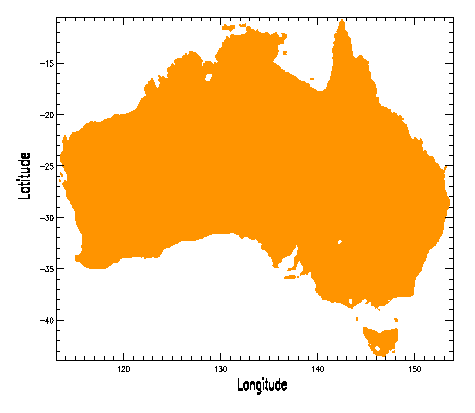
\includegraphics{Figures/check_access-a_lsm_contour}
\par\end{centering}

\caption{Plot of the land-sea mask variable, illustrating the ACCESS-A model
domain utilised in Part 2. Domain derived from the ACCESS-A Austral
region and filtered for continental regions of interest.\label{fig:ACCESS-Domain-Land-Sea}}
\end{figure}


Once the Australian continental region was defined the next step was
to extract the wind speed and Downward Shortwave Radiation (DSR) values
from the output. The DSR data was taken `as is' and without any post-processing,
however, the wind speed data needed interpolation to 80m---as per
Part 1---in order to obtain wind speed values that were at approximate
hub-height for the wind speed-power conversion. The gridding used
in the ACCESS model staggered the zonal (u) and meridional (v) components
of the wind speed via the Arakawa-C grid staggering approach (\citealp{Arakawa1977}).
The combination of the u and v components of the wind speed field
therefore involved the centering of the two fields, matching the coordinate
for the surface grid. The centring (averaging over the two adjacent
points) was necessary in order to interpolate to 80m, which involved
using the topography height on the surface grid and the height of
the pressure levels in order to determine 80m above ground level.
Once centred, the u and v components were combined to give wind speed,
as per the formula for finding the length of a vector from its base
coordinates (square-root of the sum of squares). 

This process of combining the u and v components was completed for
all levels of the ACCESS-A model output and all continental locations.
The data were then interpolated to 80m via a cubic spline through
the first five vertical levels using the height of each level in metres
above sea-level (the heights given were in geopotential height, which
is relative to sea-level) and the knowledge of the height above sea-level
of the topography from the surface files. A record of the 80m wind
speed at each continental location of interest (the domain defined
in Fig. \ref{fig:ACCESS-Domain-Land-Sea}) and the corresponding DSR
values was then formed---the 80m wind speed data were now also at
surface locations following the centring process. 

The next step in the preparation of the wind and solar data for input
into the electricity optimisation was the conversion to electricity
(in the case of wind) or electricity potential (in the case of solar).
The conversion to power output for the wind speed was conducted in
the same manner as Part 1 whereby the GE 2.5MW (see Fig. \ref{fig:GE-2.5-Power-Curve}
from Part 1) wind speed power curve was applied to all required values
of hub-height wind speed (only those locations utilised following
the site selection process outlined later). The same approach from
Part 1 was also used in terms of the input of solar radiation data
to the electricity model. No pre-determination of the solar electricity
type (photo-voltaic, concentrating solar thermal, utility-scale photo-voltaic,
or others) was made, simply a measure of solar availability was utilised.
All locations that were chosen for input into the electricity model
had their DSR values at all times converted to a percentage of maximum.
The maximum was taken as the maximum value of DSR from the ACCESS-A
data (1184.3 Wm\textsuperscript{-2}). This conversion to solar availability
(and then multiplying by the size of the installation) was noted in
\citet{Hoevenaars2012} as producing very similar values of total
output when compared to using actual output from a solar installation.
\citet{Hoevenaars2012} noted that observations at the surface can
provide a good estimate of the best-case scenario photo-voltaic installation
fitted with maximum power point tracking technology. 


\subsection{Demand Data and Preparation}

Another key component to this thesis is the use of demand data. Integral
to the usefulness of renewable electricity output is the comparison
in output with some sort of demand for the electricity that they provide.
It is a key assumption of this thesis that the combination of wind
and solar be utilised in some form to provide electricity for society
and thus any features in their combined variance that miss-match that
of demand are also vitally important. The demand data utilised in
this thesis come from two main sources---the Australian Electricity
Market Operator (AEMO), as per Part 1, and the Independent Market
Operator of Western Australia \nomenclature{IMOWA}{Independent Market Operator of Western Australia}(IMOWA).
Initially, this thesis examines the whole of Australia in terms of
the major population centres (eastern states and then Perth in WA).
In order to combine the data from IMOWA and AEMO a conversion from
local time (AEST and AWST) to all data at AEST was conducted. 

Once standardised in the temporal domain, the so called \textquoteleft{}copper-plate\textquoteright{}
combination of data was implemented. As per previous studies of renewable
electricity in this region (for instance \citet{Elliston2012}) the
copper-plate combination involved simply combining the data for all
locations---irrespective of whether or not that demand is being met
by resources in that location---thus creating a single time series
of demand for all of Australia. This time series is then used in the
Electricity Model section (Chpt. \ref{chap:The-Energy-Model}) to
compare with possible combinations of wind and solar. 

It should be noted there were also some missing data issues with the
demand data and these missing data were also assigned the value of
\textquoteleft{}NaN\textquoteright{}. Following this it was then possible
to determine the locations of missing data from all data-sets. Each
time series then had their data (either meteorological or demand)
filtered such that the temporal coverage was concordant---an important
consideration for later steps that involve optimising the wind and
solar fields to meet demand.


\section{Conclusions\label{sec:Conclusion-high-activity}}

This chapter presented an overview of the literature in the areas
of optimisation, renewable energy optimisation, and more specifically
the area of renewable energy optimisation for Australia. It was shown
that many different approaches exist for finding the optimum combination
of renewable resources (optimisation type, data used, domain used,
etc.). Specifically, there are challenges in finding the strategic
combination that maximises the percentage contribution from renewable
energy. It was also shown that there exists a high potential for Australia,
and even the large areas of the rest of the world, to rely heavily
(up to 100\%) on renewable technology. However, there is still little
known about the specific influences that the common synoptic weather
regimes will have on a high renewable energy dependent Australia.
While \citet{Elliston2012} and \citet{AEMO2013} analysed challenging
aspects to a highly renewable NEM (weeks or moments where concurrent
minima in renewable output resulted in a reliance on dispatchable
back-up generation or load shifting), the specifics regarding the
influence of meteorological drivers and their commonness, or not,
remains unexplored. This chapter also presented the data utilised
in Part 2 of this thesis. In particular, the meteorological and demand
data were shown to be relevant to this thesis and the preparation
of the data for later use was outlined. 
\end{document}
